\usepackage{amssymb, amsmath, amsbsy, amsfonts}
\usepackage[utf8]{inputenc}
\usepackage{listings}
\usepackage{emptypage}
\usepackage{caption}
\usepackage[bf,SL,BF]{subfigure}
\usepackage{mathdots}
\usepackage{mathrsfs}
\usepackage{fancyhdr}
\usepackage{eucal}
\usepackage[spanish,mexico]{babel}
\usepackage{color}
\usepackage[perpage]{footmisc}
\usepackage[sort, numbers, square]{natbib}
\usepackage{ifthen}
\usepackage{multicol}
\usepackage[nottoc]{tocbibind}
\usepackage{titlesec}
\usepackage[export]{adjustbox}

%%%%%%%%%%%%%%%%%%%%%%%%%%%%%%%%%%%%%%%%%%%%%%%%%%%%%%%%%%%%%%%%%%%%%%%%%%%%%%%%
%                         FORMATO DE TESIS UMSNH                               %
%%%%%%%%%%%%%%%%%%%%%%%%%%%%%%%%%%%%%%%%%%%%%%%%%%%%%%%%%%%%%%%%%%%%%%%%%%%%%%%%
% based on Harish Bhanderi's PhD/MPhil template, then Uni Cambridge


\documentclass[twoside,11pt]{Latex/Classes/PhDthesisPSnPDF} % "thesisUMSNH" para formato de la UMSNH
%         PUEDEN INCLUIR EN ESTE ESPACIO LOS PAQUETES EXTRA, O BIEN, EN EL ARCHIVO "PhDthesisPSnPDF.cls" EN "./Latex/Classes/"

% Estos paquetes son opcionales y a necesidad de cada quien:
\usepackage{blindtext}                             % Para insertar texto dummy, de ejemplo, pues.
\usepackage{amssymb, amsmath, amsbsy, amsfonts}    % ECUACIONES Y SÍMBOLOS MATEMÁTICOS
\usepackage{listings}                    % PERMITE AGREGAR CÓDIGO DE LENGUAJES  DE PROGRAMACIÓN (DOCUMENTACIÓN EN GOOGLE)
\usepackage{mathdots}                    % para el comando \iddots
\usepackage{mathrsfs}                    % para formato de letra en ecuaciones
\usepackage[sort, numbers]{natbib}  % Personalizar la bibliografía a gusto de cada quien

\usepackage{algpseudocode}
\usepackage{algorithmic}
\usepackage[Algoritmo]{algorithm}

% Note:
% The \blindtext or \Blindtext commands throughout this template generate dummy text
% to fill the template out. These commands should all be removed when 
% writing thesis content.


% This file contains macros that can be called up from connected TeX files
% It helps to summarise repeated code, e.g. figure insertion (see below).

%%%%%%%%%%%%%%%%%%%%%%%%%%%%%%%%%%%%%%%%%%%%%%
%            Colores de la UNAM              %
%%%%%%%%%%%%%%%%%%%%%%%%%%%%%%%%%%%%%%%%%%%%%%
% Para UNAN: Azul Pantone 655C-->(0,3,84) RGB
% Para UMSNH: PANTONE Blue 072 C
\definecolor{Azul}{RGB}{0,3,84}

% Para UNAM: Oro PANTONE 871C-->(137,118,75) RGB
% Para UMNSH: PANTONE 110 C
\definecolor{Oro}{RGB}{137,118,75}


%%%%%%%%%%%%%%%%%%%%%%%%%%%%%%%%%%%%%%%%%%%%%%
%            Comandos para líneas            %
%%%%%%%%%%%%%%%%%%%%%%%%%%%%%%%%%%%%%%%%%%%%%%
%Se define un comando \colorvrule para hacer líneas verticales de color con 3 argumentos: color, ancho, alto
\newcommand{\colorvrule}[3]{
\begingroup\color{#1}\vrule width#2 height#3
\endgroup}

%Se define un comando \colorhrule para hacer líneas horizontales de color con 2 argumentos: color, ancho
\newcommand{\colorhrule}[2]{
\begingroup\color{#1}\hrule height#2
\endgroup}

%%%%%%%%%%%%%%%%%%%%%%%%%%%%%%%%%%%%%%%%%%%%%%
%          Comando para derivadas            %
%%%%%%%%%%%%%%%%%%%%%%%%%%%%%%%%%%%%%%%%%%%%%%
\newcommand{\derivada}[3][]{\ensuremath{\dfrac{\mbox{d}^{#1}#2}{\mbox{d}#3^{#1}}}} 
%primer argumento(opcional): orden de la derivada
%segundo argumento: función a derivar
%tercer argumento: variable respecto a la que se deriva


%%%%%%%%%%%%%%%%%%%%%%%%%%%%%%%%%%%%%%%%%%%%%%
%       Comando para la exponencial          %
%%%%%%%%%%%%%%%%%%%%%%%%%%%%%%%%%%%%%%%%%%%%%%
\newcommand{\e}[1][]{\ensuremath{\mbox{e}^{#1}}}
%primer argumento(opcional): exponente de la exponencial




% insert a centered figure with caption and description
% parameters 1:filename, 2:title, 3:description and label
\newcommand{\figuremacro}[3]{
	\begin{figure}[htbp]
		\centering
		\includegraphics[width=1\textwidth]{#1}
		\caption[#2]{\textbf{#2} - #3}
		\label{condicion}
	\end{figure}
}

% insert a centered figure with caption and description AND WIDTH
% parameters 1:filename, 2:title, 3:description and label, 4: textwidth
% textwidth 1 means as text, 0.5 means half the width of the text
\newcommand{\figuremacroW}[4]{
	\begin{figure}[htbp]
		\centering
		\includegraphics[width=#4\textwidth]{#1}
		\caption[#2]{\textbf{#2} - #3}
		\label{#1}
	\end{figure}
}

% inserts a figure with wrapped around text; only suitable for NARROW figs
% o is for outside on a double paged document; others: l, r, i(inside)
% text and figure will each be half of the document width
% note: long captions often crash with adjacent content; take care
% in general: above 2 macro produce more reliable layout
\newcommand{\figuremacroN}[3]{
	\begin{wrapfigure}{o}{0.5\textwidth}
		\centering
		\includegraphics[width=0.48\textwidth]{#1}
		\caption[#2]{{\small\textbf{#2} - #3}}
		\label{#1}
	\end{wrapfigure}
}

% predefined commands by Harish
\newcommand{\PdfPsText}[2]{
  \ifpdf
     #1
  \else
     #2
  \fi
}

\newcommand{\IncludeGraphicsH}[3]{
  \PdfPsText{\includegraphics[height=#2]{#1}}{\includegraphics[bb = #3, height=#2]{#1}}
}

\newcommand{\IncludeGraphicsW}[3]{
  \PdfPsText{\includegraphics[width=#2]{#1}}{\includegraphics[bb = #3, width=#2]{#1}}
}

\newcommand{\InsertFig}[3]{
  \begin{figure}[!htbp]
    \begin{center}
      \leavevmode
      #1
      \caption{#2}
      \label{#3}
    \end{center}
  \end{figure}
}







%%% Local Variables:
%%% mode: latex
%%% TeX-master: "~/Documents/LaTeX/CUEDThesisPSnPDF/thesis"
%%% End:
           % Archivo con funciones útiles





%%%%%%%%%%%%%%%%%%%%%%%%%%%%%%%%%%%%%%%%%%%%%%%%%%%%%%%%%%%%%%%%%%%%%%%%%%%%%%%%
%                                   DATOS                                      %
%%%%%%%%%%%%%%%%%%%%%%%%%%%%%%%%%%%%%%%%%%%%%%%%%%%%%%%%%%%%%%%%%%%%%%%%%%%%%%%%
\title{Inteligencia Artifical para la Caracterización de Rayos Cósmicos en Detectores RICH}
\author{José Daniel Bazán Manzano} 
\facultad{Facultad de Ciencias}                 % Nombre de la facultad/escuela
\escudofacultad{Latex/Classes/Escudos/fc_azul} % Aquí ponen la ruta y nombre del escudo de su facultad, actualmente, la carpeta Latex/Classes/Escudos cuenta con los siguientes escudos:
% "fi_azul" Facultad de ingenieria en color azul
% "fi_negro" Facultad de ingenieria en color negro
% "fc_azul" Facultad de ciencias en color azul
% "fc_negro" Facultad de ciencias en color negro
% "fmed_grande" Facultad de medicina UMSNH
% Se agradecen sus aportaciones de escudos a jebus.velazquez@gmail.com

\degree{Físico}       % Carrera
\director{Dr. Diego Mauricio Gómez Coral}                 % Director de tesis
%\tutor{Nombre  Tutor }                    % Tutor de tesis, si aplica
\degreedate{2024}                          % Año de la fecha del examen
\lugar{Ciudad Universitaria, CDMX}         % Lugar

%\portadafalse                              % Portada en NEGRO, descomentar y comentar la línea siguiente si se quiere utilizar
\portadatrue                                % Portada en COLOR



%% Opciones del posgrado (descomentar si las necesitan)
	%\posgradotrue                                                    
	%\programa{programa de maestría y doctorado en ingeniería}
	%\campo{Ingeniería Eléctrica - Control}
	%% En caso de que haya comité tutor
	%\comitetrue
	%\ctutoruno{Dr. Emmet L. Brown}
	%\ctutordos{Dr. El Doctor}
%% Datos del jurado                             
	%\presidente{Dr. 1}
	%\secretario{Dr. 2}
	%\vocal{Dr. 3}
	%\supuno{Dr. 4}
	%\supdos{Dr. 5}
	%\institucion{el Instituto de Ingeniería, UNAM}

\keywords{tesis,autor,tutor,etc}            % Palablas clave para los metadatos del PDF
\subject{tema_1,tema_2}                     % Tema para metadatos del PDF  

%%%%%%%%%%%%%%%%%%%%%%%%%%%%%%%%%%%%%%%%%%%%%%%%%%%%%
%                   PORTADA                         %
%%%%%%%%%%%%%%%%%%%%%%%%%%%%%%%%%%%%%%%%%%%%%%%%%%%%%
\begin{document}

\maketitle									% Se redefinió este comando en el archivo de la clase para generar automáticamente la portada a partir de los datos

%%%%%%%%%%%%%%%%%%%%%%%%%%%%%%%%%%%%%%%%%%%%%%%%%%%%%
%                  PRÓLOGO                          %
%%%%%%%%%%%%%%%%%%%%%%%%%%%%%%%%%%%%%%%%%%%%%%%%%%%%%
\frontmatter
\begin{dedication}
Al Dr. Diego que me ha instruido en los inquietantes mundos de la academia y por su apoyo, a Yunué por todo y a mi Mama por que sin Ella no hubiera sido posible este trabajo.\\
Su Servidor.
\end{dedication}
       % Comentar línea si no se usa
%\chapter*{}
%\pagenumbering{Roman}

\begin{acknowledgements}

También quisiera reconocer a PAPIIT ya que me otorgó una beca para la realización de este trabjo y ...
\end{acknowledgements}




   % Comentar línea si no se usa 
% ******************************* Thesis Declaration ********************************

\begin{declaration}

Por la presente declaro que, salvo cuando se haga referencia específica al trabajo de otras personas, el contenido de esta tesis es original y no se ha presentado total o parcialmente para su consideración para cualquier otro título o grado en esta o cualquier otra Universidad. Esta tesis es resultado de mi propio trabajo y no incluye nada que sea el resultado de algún trabajo realizado en colaboración, salvo que se indique específicamente en el texto. 
% Author and date will be inserted automatically from thesis.tex


\end{declaration}
           % Comentar línea si no se usa

% Thesis Abstract -----------------------------------------------------


%\begin{abstractslong}    %uncommenting this line, gives a different abstract heading
\begin{abstracts}        %this creates the heading for the abstract page

En esta tesis se entrenaron Redes Neuronales para la caracterización de rayos cósmicos utilizando detectores RICH (Ring Imaging Cherenkov). Los rayos cósmicos, partículas que permean el universo, pueden proporcionar información valiosa sobre la anturaleza de los antinúcleos detectados por el experimento AMS-02 proporcionado un entendimiento sobre la asimetría materia-antimateria. El objetivo principal es desarrollar y aplicar IA para contrastarla con algoritmos de verosimilitud -El método del estado del arte en RICH-  la precisión y eficiencia en la identificación y análisis de estos rayos.

Las técnicas de inteligencia artificial implementadas en este estudio demuestran una mejora significativa en la caracterización de los rayos cósmicos comparadas con los métodos tradicionales. Los resultados refuerzan la noción que la inteligencia artificial puede auxiliar significativamente la detección y análisis de partículas en futuros experimentos de física de partículas y astrofísica. Este trabajo plantea  un modelo eficiente y rápido, sugiriendo la continuación de esta línea de investigación para perfeccionar y ampliar sus aplicaciones.



\end{abstracts}
%\end{abstractlongs}


% ----------------------------------------------------------------------                   % Comentar línea si no se usa

%%%%%%%%%%%%%%%%%%%%%%%%%%%%%%%%%%%%%%%%%%%%%%%%%%%%%
%                   ÍNDICES                         %
%%%%%%%%%%%%%%%%%%%%%%%%%%%%%%%%%%%%%%%%%%%%%%%%%%%%%
%Esta sección genera el índice
\setcounter{secnumdepth}{3} % organisational level that receives a numbers
\setcounter{tocdepth}{3}    % print table of contents for level 3
\tableofcontents            % Genera el índice 
%: ----------------------- list of figures/tables ------------------------
\listoffigures              % Genera el ínidce de figuras, comentar línea si no se usa
\listoftables               % Genera índice de tablas, comentar línea si no se usa


%%%%%%%%%%%%%%%%%%%%%%%%%%%%%%%%%%%%%%%%%%%%%%%%%%%%%
%                   CONTENIDO                       %
%%%%%%%%%%%%%%%%%%%%%%%%%%%%%%%%%%%%%%%%%%%%%%%%%%%%%
% the main text starts here with the introduction, 1st chapter,...
\mainmatter
\def\baselinestretch{1.5}                   % Interlineado de 1.5

% this file is called up by thesis.tex
% content in this file will be fed into the main document
%----------------------- introduction file header -----------------------
%%%%%%%%%%%%%%%%%%%%%%%%%%%%%%%%%%%%%%%%%%%%%%%%%%%%%%%%%%%%%%%%%%%%%%%%%
%  Capítulo 1: Introducción- DEFINIR OBJETIVOS DE LA TESIS              %
%%%%%%%%%%%%%%%%%%%%%%%%%%%%%%%%%%%%%%%%%%%%%%%%%%%%%%%%%%%%%%%%%%%%%%%%%

\chapter{Introducción}

%: ----------------------- HELP: latex document organisation
% the commands below help you to subdivide and organise your thesis
%    \chapter{}       = level 1, top level
%    \section{}       = level 2
%    \subsection{}    = level 3
%    \subsubsection{} = level 4
%%%%%%%%%%%%%%%%%%%%%%%%%%%%%%%%%%%%%%%%%%%%%%%%%%%%%%%%%%%%%%%%%%%%%%%%%
%                           Presentación                                %
%%%%%%%%%%%%%%%%%%%%%%%%%%%%%%%%%%%%%%%%%%%%%%%%%%%%%%%%%%%%%%%%%%%%%%%%%

\section{Presentación} % section headings are printed smaller than chapter names
\blindtext
%%%%%%%%%%%%%%%%%%%%%%%%%%%%%%%%%%%%%%%%%%%%%%%%%%%%%%%%%%%%%%%%%%%%%%%%%
%                           Objetivo                                    %
%%%%%%%%%%%%%%%%%%%%%%%%%%%%%%%%%%%%%%%%%%%%%%%%%%%%%%%%%%%%%%%%%%%%%%%%%

\section{Objetivo}

Este trabajo tiene por objetivo ...
\blindtext
%%%%%%%%%%%%%%%%%%%%%%%%%%%%%%%%%%%%%%%%%%%%%%%%%%%%%%%%%%%%%%%%%%%%%%%%%
%                           Motivación y estado del arte                %
%%%%%%%%%%%%%%%%%%%%%%%%%%%%%%%%%%%%%%%%%%%%%%%%%%%%%%%%%%%%%%%%%%%%%%%%%
\section{Motivación}


\blindtext
%%%%%%%%%%%%%%%%%%%%%%%%%%%%%%%%%%%%%%%%%%%%%%%%%%%%%%%%%%%%%%%%%%%%%%%%%
%                   Planteamiento del problema                          %
%%%%%%%%%%%%%%%%%%%%%%%%%%%%%%%%%%%%%%%%%%%%%%%%%%%%%%%%%%%%%%%%%%%%%%%%%

\section{Planteamiento del problema}
\blindtext
%%%%%%%%%%%%%%%%%%%%%%%%%%%%%%%%%%%%%%%%%%%%%%%%%%%%%%%%%%%%%%%%%%%%%%%%%
%                           Metodología                                 %
%%%%%%%%%%%%%%%%%%%%%%%%%%%%%%%%%%%%%%%%%%%%%%%%%%%%%%%%%%%%%%%%%%%%%%%%%
\section{Metodología}

Se tiene un objetivo principal, y para llegar a \'el %otra forma de poenr acentos
\blindtext
%%%%%%%%%%%%%%%%%%%%%%%%%%%%%%%%%%%%%%%%%%%%%%%%%%%%%%%%%%%%%%%%%%%%%%%%%
%                         Contribuciones                                %
%%%%%%%%%%%%%%%%%%%%%%%%%%%%%%%%%%%%%%%%%%%%%%%%%%%%%%%%%%%%%%%%%%%%%%%%%

\section{Contribuciones}

La principal contribución de este trabajo es 
\blindtext
%%%%%%%%%%%%%%%%%%%%%%%%%%%%%%%%%%%%%%%%%%%%%%%%%%%%%%%%%%%%%%%%%%%%%%%%%
%                           Estructura de la tesis                      %
%%%%%%%%%%%%%%%%%%%%%%%%%%%%%%%%%%%%%%%%%%%%%%%%%%%%%%%%%%%%%%%%%%%%%%%%%

\section{Estructura de la tesis}

Este trabajo está dividido en XX capítulos. Al principio se encuentra 
\\\\
Finalmente se encuentra la parte de             % ~10 páginas - Explicar el propósito de la tesis

%%%%%%%%%%%%%%%%%%%%%%%%%%%%%%%%%%%%%%%%%%%%%%%%%%%%%%%%%%%%%%%%%%%%%%%%%
%           Capítulo 2: MARCO TEÓRICO - REVISIÓN DE LITERATURA
%%%%%%%%%%%%%%%%%%%%%%%%%%%%%%%%%%%%%%%%%%%%%%%%%%%%%%%%%%%%%%%%%%%%%%%%%

\chapter{La Asimetría Bariónica y el Experimento AMS-02}
\section{Nucleosíntesis del Big Bang}


\section{Rayos cósmicos}

\begin{figure}[h!]
    \centering
    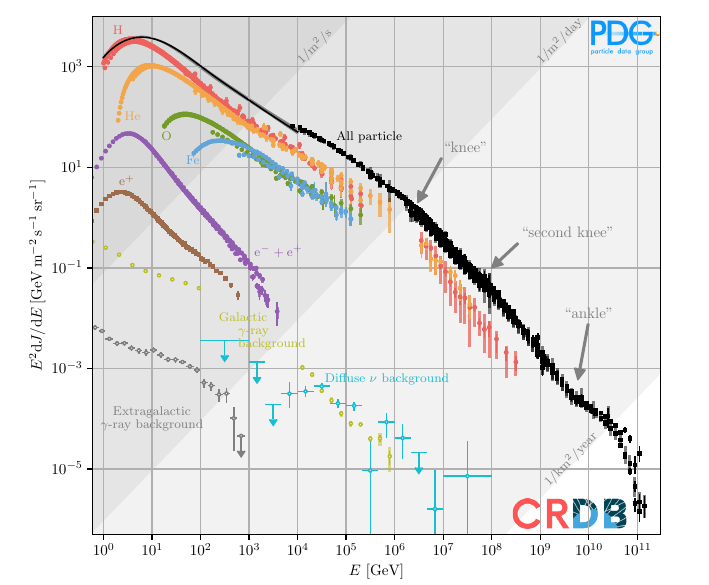
\includegraphics[scale=0.6]{Tesis-UNAM/Capitulo2/RCespectro.png}
    \caption{Espectro de los RC's}
    \label{fig:enter-label}
\end{figure}
Los Rayos Cósmicos(RC) son un conjunto de partículas no termales que permean el universo, una forma de caracterizar los RC es a través de su espectro, composición y su distribución espacial. Para RC cargados, por ejemplo, su espectro se extiende desde unas decenas de MeV's a casi 1 ZeV. La distribución espectral obedece diferentes leyes de potencias i.e. $E^{-\gamma}$\cite{Workman:2022ynf}. Dependiendo del rango de energía el factor $\gamma$ cambia, lo que da a lugar a decir que presenta varias estructuras. Para energías menores a unos cuantos PeV, el indice espectral $\gamma \approx 2.7$, a mayores energías el indice cambia a ~3, esta estructura se le llama la rodilla, para energías encontramos la segunda rodilla, donde $\gamma \approx3.3$ y por último los RC más energéticos que 1 EeV $\gamma \approx2.5$ forman una estructura denominada "tobillo"\cite{Workman:2022ynf}.\\

La composición de los RC consiste mayormente en protones, helio y demás nucleos, aun que también se encuentran positrones, electrones, antiprotones, y recientemente el experimento AMS ha detectado antinucleos\cite{Doetinchem_2020}. La distribución espacial es mayormente isotrópica, aun que debido al campo magnético galáctico y la disposición de las fuentes se han observado anisotropias alrededor de la "rodilla"\cite{Workman:2022ynf}; además de los RC cargados, rayos gamma y neutrinos altamente energéticos también componen parte de los RC.\\

Los RC cargados son desviados numerosas ocasiones por varios campos magnéticos, así que la dirección en la que son detectados no apunta hacía su fuente\cite{Workman:2022ynf}. Dependiendo de la energía se piensa que los RC son galácticos ($<$PeV) y extragalácticos ($>$EeV).\cite{Workman:2022ynf}\\

Algunos posibles candidatos a fuentes se asocian principalmente a las últimas etapas de la vida estelar, o a agujeros negros supermasivos que emiten gran cantidad de energía rotacional y gravitatoria\cite{Workman:2022ynf}. Se ha pensado como posibles fuentes galácticas a microcuásares, el centro de la via láctea, o viento estelar de clusteres de estrellas, mientras que para las extragalácticas se piensa que son núcleos galácticos activos, pulsares, magnetares y galaxias con brotes estelares\cite{Workman:2022ynf}.\\

\begin{figure}
    \centering
    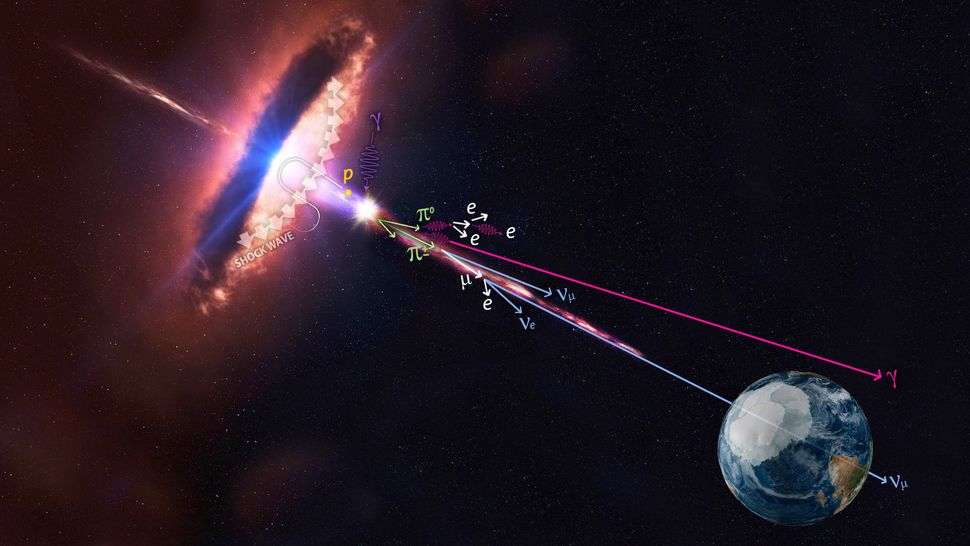
\includegraphics{Tesis-UNAM/Capitulo2/cosmicRays.jpg}
    \caption{Diagrama Ilustrativo de Los Rayos Cósmicos y sus Fuentes}
    \label{fig:enter-label}
\end{figure}

Dentro de la Vía Láctea, el proceso de transporte más importante de los rayos cósmicos es la difusión\cite{Workman:2022ynf}, cómo lo demuestran las anisotropías en las direcciónes de llegada y mayor abundancia de algunas especies nucleares, este mecanismo difusivo se debe a las múltiples interacciones de los RC cargados con los campos magnéticos presentes en el Universo. Aun que también otros procesos contribuyen al transporte observado, cómo son, perdidas de momento, perdidas radiativas, ionización, espalación (creación de nucleos más ligeros a partir de colisiones inelásticas)\cite{Workman:2022ynf}. \\

El estudio de los rayos cósmicos puede ser provechoso para la comprensión de fenómenos astrofísicos, ya que constituyen una parte muy considerable del contenido energético en varios ambientes en el Universo. La presión de los RC es tal que pueden modificar su entorno, e.g. Los RC contribuyen a la estructura gravitacional de las galaxias, y pueden impulsar flujos de salida en escalas galácticas. También los rayos cósmicos causan turbulencias lo que afecta en gran medida el transporte galáctico y la aceleración de choque\\

La física fundamental también se beneficia notablemente del estudio de RC, por ejemplo si la materia oscura(MO) interacciona con el modelo estandar, uno podría observar productos de auto-aniquilaciones o de decaimientos de la MO. Otro gran enigma que podrían elucidar los RC es sobre la asimetría matera-antimateria, dado que por mucho la gran mayoria de rayos cósmicos son conformados de materia ordinaria. Por último ha habido un exceso de rayos-$\gamma$ y neutrinos detectados provenientes del núcleo de la Vía Lactea, lo cuál concordaría con las predicciones de algunos modelos de MO \cite{Workman:2022ynf}\\

% Incluir información sobre antinúcleos en rayos cósmicos
% Hablar sobre su producción secundaria por rayos cósmicos con el medio interestelar y también sobre la posible producción por materia oscura
% Los antinucleos detectados por AMS


\section{Radiación Cherenkov}
\subsection{Descubrimiento}
Pavel A. Cherenkov, en los años de 1930 a 1935 realizó su doctorado sobre la luminiscencia de soluciones de sales de uranilo bajo la acción de rayos-$\gamma$, Cherenkov investigó el fenómeno de la luminiscencia inducida por rayos-$\gamma$ de una fuente de radio comparandola con la emisión de luz luminofora.\cite{CHERENKOVA20088}\\
%\subsubsection{Técnicas Experimentales}
%Para todos estos estudios se utilizaron dos fuentes unicamente, rayos X y luz visible y dado que la intensidad de la luz fué mínima, se requería un diseño de un dispositivo de fotometría lo suficientemente sensible para poder realizar mediciones cuantitativas; Cherenkov se decidió por una cuña óptica con el ojo humano cómo detector óptico. \\

%El montaje experimental se describe en la figura 2.1, el recipiente A con el líquido luminóforo y la fuente radioactiva se posan sobre un soporte B, el espesor promedio del recipiente son tales que la radiación $\alpha$ y $\beta$ sea absorbida pero los rayos-$\gamma$ puedan atraversar el contenedor, el soporte B poseé dos ranuras $R_1$ y $N_2$ donde se colocaron pequeñas muesras de radio el prisma nicol $N$ se puede utilizar para realizar medidas sobre la polarización de la luz, también se utilizo un colimador $L_1$ un prisma P, un telescopio formado por dos lentes $L_1$ y $L_2$ y la cuña óptica K, varios filtros ópticos se pueden montar en el marco E, y el diafragma D define el campo de visión.
%A pesar de la simplesa del diseño experimental, Cherenkov pudo realizar las mediciones con una alta precisión.
%\begin{figure}[h!]
    %\centering
    %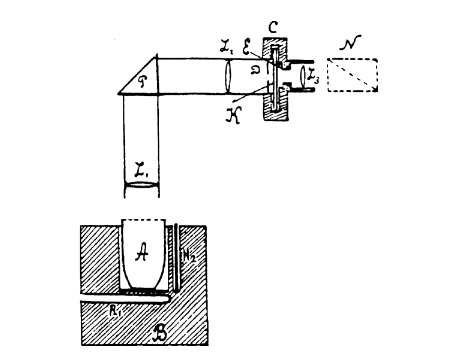
\includegraphics[scale=0.6]{Tesis-UNAM/Capitulo2/experimentoCerenkov.png}
    %\caption{Esquema del montaje experimental}
    %\label{fig:enter-label}
%\end{figure}
%\\\\%

Al realizar sus experimentos en luminiscencia, Cherenkov se dió cuenta de un fenómeno peculiar, al incidir rayos-$\gamma$ sobre ácido sulfúrico\cite{CHERENKOVA20088}, se presentaba una pequeña emisión de luz azul, hoy sabemos que esto fue radiación cherenkov emitida a causa de electrones acelerados por dispersión compton debida a los rayos-$\gamma$. También se estudió la polarización de esta radiación electromagnética\cite{Bashmakov_2015}, bajo condiciones óptimas se obtuvo un 20$\%$ de polarización total, donde el plano dominante del campo eléctrico era paralelo a la dirección de propagación de los rayos-$\gamma$. \\\\
En posteriores experimentos Cherenkov implementó una geometría axiosimétrica, un contenedor cilíndrico transparente con el líquido a estudiar, se rodeó de un espejo con una geometría cónica, subsecuentemente el recipiente se cubrió con una cubierta que no era transparente a la luz, y la fuente radioactiva se colocaba en el exterior del espejo\cite{Bashmakov_2015}. Gracias a estas investigaciones se descubrió una de las características más interesantes de esta emisión lumínica, la cuál la diferencían de las radiaciones previamente conocidas a los estudios de Cherenkov - su asimetría espacial\cite{Bashmakov_2015}. Este descurbrimiento le valió el Premio Nóbel de Física de 1958 a Cherenkov.

\subsection{Descripción y Naturaleza del Fenómeno}
La descripción teórica del fenómeno fue desarrollada por I.M. Frank e I.E. Tamm\cite{Bashmakov_2015, Jelley, CHERENKOVA20088}, la cual fue verificada posteriormente por P. Cherenkov. Donde hicieron una analogía con las ondas Mach de la hidrodinámica (Aunque Sommerfeld y Heaviside ya habian predicho la emisión de luz por partículas cargadas moviendose a velocidades supralumínicas previamente)\cite{CHERENKOVA20088, Bashmakov_2015}. \\\\
Una forma de entender el fenómeno parte de la electrodinámica clásica, en donde se calcula que el campo eléctrico de una partícula cargada moviendose a una velocidad cercana a la de la luz poseé una forma parecida a la de un disco plano\cite{Bashmakov_2015, Jelley, Beyer}. \\\\

\begin{figure}[h!]
    \centering
    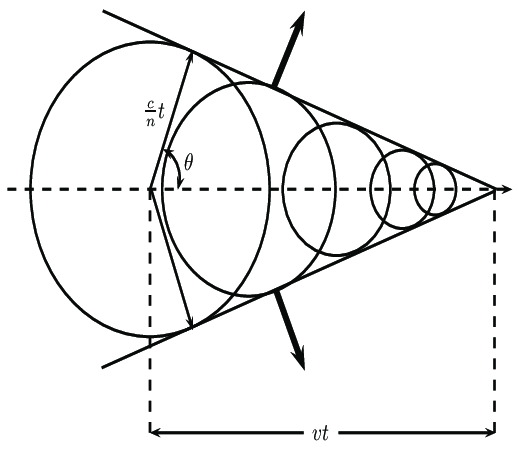
\includegraphics[scale=0.5]{Tesis-UNAM/Capitulo2/Figura-26-Representacion-pictorica-del-proceso-de-emision-de-radiacion-de-Cherenkov-La.png}
    \caption{Descripción bajo el esquema electrodinámico de la radiación Cherenkov}
    \label{fig:enter-label}
\end{figure}


El plano de el disco es perpendicular a la dirección del desplazamiento de la partícula, esta distribución es axisimétrica con respecto al vector de velocidad y simétrica con el plano medio del disco. Este campo eléctrico puede ser descrito como una superposición de ondas electromagnéticas planas, con estas consideraciones uno puede definir varios fotones virtuales con vectores de onda $\Vec{k}$ paralelos a $\Vec{v}$, y la componente transversal $\Vec{k}_\perp$ es cero\cite{Bashmakov_2015}.\\\\
Si la partícula se mueve a una velocidad mayor que la de la luz en el medio, el campo eléctrico en frente de la carga será nulo, la simetría axial se mantiene pero la distribución del campo eléctrico cambia a la de un cono. En la figura 2.2 se puede observar graficamente lo descrito anteriormente.\cite{Bashmakov_2015, Jelley}


\subsubsection{Mecanismos Físicos}
Debido al campo eléctrico generado por el movimiento de la partícula cargada, la distribución electrónica de las moléculas de la materia se verá afectada, causando que aparezcan diversos dipolos localizados en las inmediaciones de la partícula en movimiento\cite{Beyer, Jelley}. Cuando su velocidad es muy pequeña la distribución de estos dipolos es simétrica, pero al superar el umbral de la velocidad de la luz sobre el medio, debido al potencial retardado, la deformación de los orbitales electrónicos se vuelve asimétrica (fig 2.3), causando un campo dipolar resultante aun en puntos distantes de la carga. Cada uno de estos dipolos radiaran cómo una antena\cite{Beyer, Jelley}.\\

\begin{figure}[h!]
    \centering
    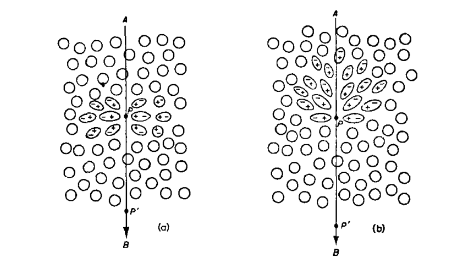
\includegraphics{Tesis-UNAM/Capitulo2/dipole.png}
    \caption{(a) Partícula con una velocidad baja (b) Partícula viajando a una velocidad mayor que la de la luz en el medio}
    \label{fig:enter-label}
\end{figure}

En un caso más realista el material tendrá un grosor considerable, esto implicará que los dipolos a lo largo de la trayectoria radien de forma sucesiva, aunque de tal forma que haya interferencia y que la emisión se propague en un ángulo fijo\cite{Jelley, Beyer}\\.

Usando esto como fundamento, Tamm y Frank pudieron mostrar\cite{Bashmakov_2015, Jelley, Beyer} que una partícula con carga Z que se mueve a una velocidad $v = \beta c$ en un medio con un indice de refracción $n\omega$ emitirá N fotones por cm recorrido en el medio en un intervalo de frecuencias $d\omega$

$$N(\omega)d\omega = \frac{2\pi Z^2 e^2}{\hbar c^2}\left(1 - \frac{1}{\beta^2n_\omega^2} \right)d\omega$$

Donde la emisión para una frecuencia específica se transmite en un ángulo Cerenkov determinado por la ecuación \cite{Bashmakov_2015, Jelley}

\begin{equation}
    cos\theta_\omega = \frac{1}{\beta n_\omega}
\end{equation}


\section{Detectores Cerenkov}

%Profundizar más, buscar bibliografía que te ayude
% Incluir efectos de dispersión y entender y explicar la física del proceso


\begin{figure}
    \centering
    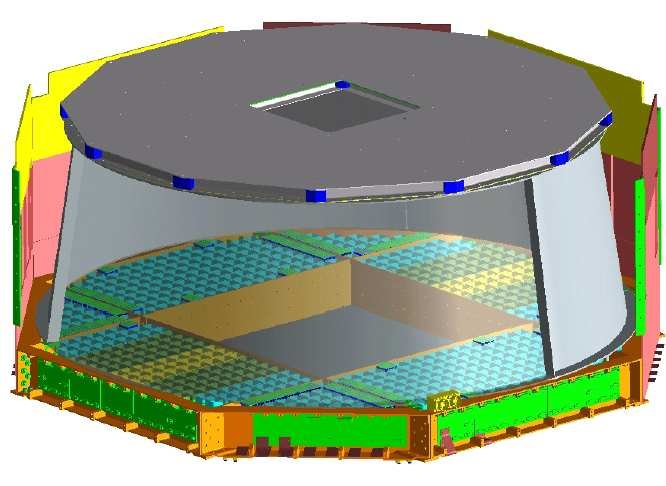
\includegraphics[scale=0.4]{Tesis-UNAM/Capitulo2/The-RICH-detector-of-AMS-02-left-View-of-the-assembled-RICH-detector-at-CIEMAT-right.jpg}
    \caption{Detector RICH de la misión AMS-02 \cite{AMSRICH}}
    \label{fig:enter-label}
\end{figure}

Una forma de estudiar el espectro y la composición de los rayos cósmicos es a través de la identificación de sus constituyentes y de la medición de su velocidad\cite{RICHCERN}, para esto es imprescindible el diseño de detectores con gran eficiencia. Esto es posible midiendo su masa y su carga eléctrica, a través de propiedades correlacionadas a la primera, cómo el momento la energía cinética y su velocidad $\beta$\cite{RICHCERN}, ya que si dos de ellas son medidas, se puede obtener la masa. En muchos experimentos, cómo es el caso de AMS-02, se acoplan varios detectores en conjunto, lo cuál permite cuantificar por separado las diferentes cantidades necesarias para la caracterización, e.g. la rigidez R midiendo el gyro radio de la partícula atravezando un campo magnético. Y a partir de la rigidez se obtiene el momento. Así que si consideramos un campo magnético B y el radiogiro de la partícula $\rho$

$$R = B\rho = \frac{p}{Z}$$
$$p = \gamma m_0c\beta$$
$$\Longrightarrow m_0 = \frac{RZ}{\gamma v}$$

Al obtener la masa en términos de la velocidad y el momento, uno puede ver la gran utilidad de los detectores cherenkov ya que este nos permite obtener la velocidad de la partícula, esto puede ilustrarse utilizando la ecuación (2.2) al obtener la relación entre el ángulo cherenkov y su masa.\cite{RICHCERN}

$$\frac{v}{c}=\beta=\frac{1}{n(\omega) cos\theta_\omega}$$
\begin{equation}
    \frac{RZn(\omega)}{c\gamma cos\theta}
\end{equation}

\subsection{Radiadores}
Los detectores Cerenkov son a grandes rasgos sensores de luz cerenkov emitida por partículas cargadas al atravesar un radiador, o sistema de radiadores. Estos radiadores pueden ser sólidos o gases\cite{RICHCERN}, tales que sean capaces de absorber o dispersar la menor cantidad de fotones posibles, y que dispongan con índices de refracción particulares dependiendo de la velocidad de las partículas que se pretenda caracterizar.\\

Por ejemplo, si queremos obtener $\beta$ en función del índice de refracción n, vemos el siguiente comportamiento (fig 2.4).\\

\begin{figure}[h!]
    \centering
    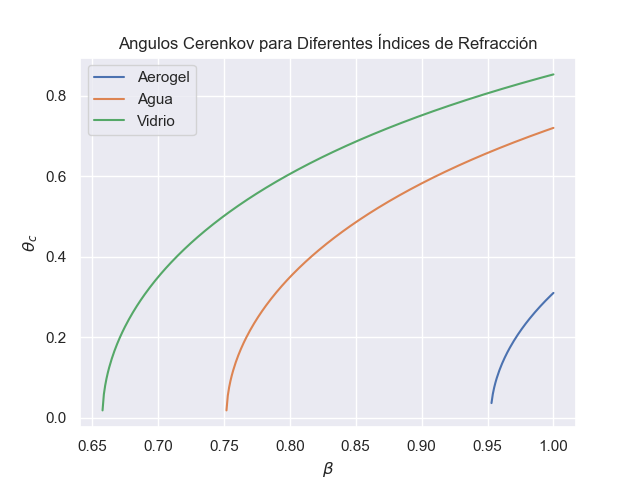
\includegraphics[scale=0.5]{Tesis-UNAM/Capitulo2/radiatorPrecision.png}
    \caption{Ángulo cerenkov contra beta}
    \label{fig:enter-label}
\end{figure}

Al incrementar la velocidad de la partícula, hasta el punto de llegar a la velocidad de la luz i.e. $\beta \longrightarrow 1$ se observa que $\theta = 1/n(\lambda)$, también se concluye que la sensibilidad es mayor al medir en angulos cerca de zonas donde $\frac{d\theta}{d\beta}$ es considerable, nótese que para protones (el cosntituyente más abundante de los rayos cósmicos) a una energía cerca de los 3-4 GeV, $\beta \approx 0.975$
el aerogel presenta una gran sensibilidad, en cambio para vidrio o agua el ángulo cerenkov empieza a saturarse más y más. Por esta razón es necesario utlizar el radiador adecuado en función de la velocidad estimada a medir por el radiador en cuestión.\\

Otras cuestiones de importancia serían que la luz cerenkov pueda atravesar el radiador con la menor perdida posible, debido a la poca cantidad de fotones emitidos por la partícula cargada en comparación a procesos centelladores, también hay que añadir que es muy importante que el radiador no centelleé de manera apreciable y además es crucial que el radiador sea transparante a la emisión cerenkov, que en la mayoría de los casos es en el rango del ultravioleta y que no haya bandas de absorción en el rango de operación\cite{RICHCERN}

\subsection{Sensores de Fotones}
El proposito fundamental de estos sensores es el de convertir la radiación cerenkov emitida por el radiador y convertirla en una señal eléctrica\cite{RICHCERN}, una consideración importante es que debido a la baja energía de los fotones cerenkov es que sólo es posible aprovechar cómo mecanismo de interacción de la luz con la materia la absorción fotoeléctrica, otra sería que el sensor debe de ostentar una eficiencia de detección alta de eléctrones individuales desprendidos de los átomos del material fotosensible.\\

Un tipo de  sensores con alta relevancia hoy en día serian los tubos PMT(Photomultiplier tubes) estos funcionan gracias al efecto fotoeléctrico. Aun que el experimento Helix tiene pensado implementar SiPM's (Silicon Photomultipliers) los cuales necesitan voltajes de polarización relativamente bajos y ostentan otra serie de ventajas e.g. un menor tamaño y peso.


%subsección
% Identificación de antinúcleos
% como se usa el RICH para identificar antinúcles a partír de la beta
% reconstrucción de masa y resolución de la masa (revisar presentaciones de ams)



\subsection{Experimentos Actuales}
En esta sección se presentará un breve recuento de los detectores RICH usados actualmante para remarcar la gran utilidad que poseen este tipo de experimentos para la física nuclear y de partículas.

\subsubsection{COMPASS} Detector RICH con radiador gaseoso de aceptancia ancha, donde se realizan detecciones de fotones únicos con detectores gaseosos y tubos fotmultiplicadores y haciendo uso de espejos esféricos. Ha conseguido la identificación de hadrones con un momento alto en el espectrometro COMPASS del CERN SPS, dedicado a estudiar la estructura hadrónica y a la espectroscopía hadrónica \cite{ALBRECHT2003112}

\subsubsection{Babar} La misión principal del experimento Babar es el estudio de las asimetrías que surgen en violaciones de la CP (paridad y carga) en el decaimiento de mesones neutrales B. Este experimento poseé el primer detector DIRC(Detector of Internally Reflected Cherenkov light), el cuál usa como radiador barras de cuarzo sumamente polidas. Se muestra un esquema de su funcionamiento.\cite{babas}

\begin{figure}[h!]
    \centering
    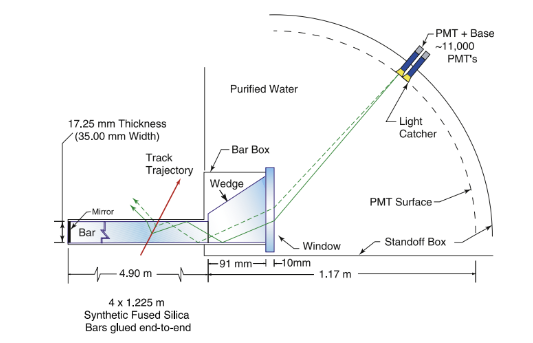
\includegraphics{Tesis-UNAM/Capitulo2/babasDirc.png}
    \caption{Caption}
    \label{DIRC del detector Babar}
\end{figure}

\subsubsection{LHCb} Una característica clave del diseño de este experimento es el de contar con dos RICH y tres tipos de radiadores aerogel, $C_4_{10}$ Y $CF_4$, el objetivo era identificar partículas con momento de 4-100 GeV/c. También cuenta con un novedoso detector de fotones, el HPD(Hybrid Pixel Detector), gracias a una considerable area sensible, se pudo obtener una buena cobertura geométrica a la vez de poder detectar una gran cantidad de fotones \cite{PAPANESTIS2020162004}

\pagebreak

\begin{figure}[h!]
    \centering
    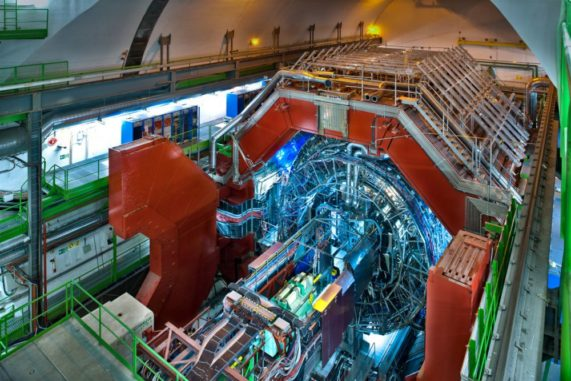
\includegraphics[scale=0.7]{Tesis-UNAM/Capitulo2/news_2765-571x381.jpg}
    \caption{Experimento ALICE}
    \label{fig:enter-label}
\end{figure}

\subsubsection{ALICE} El aparato ALICE consiste en estudiar colisiones $p^+p^+$, $p^+-Pb$ y $Pb-Pb$ proveidas por el LHC. Consiste de 7 Contadores RICH y usan $C_6F_{14}$ líquido cómo radiador, para detectar los fotones utiliza una cámara proporcional acoplada a un fotocatodo revestido de CsI \cite{VOLPE2014259}

\subsubsection{CBM} El experimento CBM está diseñado para estudiar las propiedades de la materia nuclear y mapear el diagrama de fase del QCD. E especial el RICH del CMB se planteo cómo una forma de detectar electrones con momento de hasta 8 GeV/c. Consiste de un radiador gaseoso de $CO_2$, un sistema de espejos esféricos, y de tubos fotomultiplicadores Hamamatsu \cite{ADAMCZEWSKIMUSCH201765}

\pagebreak

\subsubsection{AMS-02} 

%Profundizar en la descripción de AMS y otros experimentos de rayos cósmicos que tengan un RICH

El experimento AMS consta de un espectrómetro magnético de partículas de alta energía acoplado a la estación espacial internacional, lo que le brinda la gran ventaje de detectar rayos cósmicos sin haber interactuado con la atmósfera terreste. En el se encuentra un subdector RICH conformado de dos radiadores, uno de aerogel y otro de NaF, con tubos fotomultiplicadores. Ha sido el primer experimento en observar antinúcleos de helio. Para concluir el capítulo se tiene que enfatizar que este ha sido el detector utilizado cómo base de las simulaciones utilizadas para generar los datos a caracterizar.\cite{LIU20175}           % ~20 páginas - Poner un contexto a la tesis, hacer referencia a trabajos actuales en el tema

%%%%%%%%%%%%%%%%%%%%%%%%%%%%%%%%%%%%%%%%%%%%%%%%%%%%%%%%%%%%%%%%%%%%%%%%%
%           Capítulo 3: NOMBRE                   %
%%%%%%%%%%%%%%%%%%%%%%%%%%%%%%%%%%%%%%%%%%%%%%%%%%%%%%%%%%%%%%%%%%%%%%%%%

\chapter{Herramientas Computacionales}
Una vez entendido el funcionamiento detrás los detectores RICH y cómo pueden contribuir a la carcterización de rayos cósmicos, se procederá a explicar en detalle algunas técnicas de análisis de datos, los cuales son utilizados en este trabajo sobre el estudio de los patrones RICH.

\section{Verosimilitud}
La funcíon de verosimilitud se define cómo

\begin{equation}
    L(\theta) = p(x|\theta)
\end{equation}

donde $\theta$ es un conjunto de parámetros característicos de alguna distribución probabilistica e.g. $\sigma$ y $\mu$ para la distribución normal, y x una colección de observaciónes e.g. las posiciones de los fotones cherenkov detectados.\cite{likeCern}\\

 Uno podría interpretar la función de verosimilitud cómo la "probabilidad que una distribución de probabilidad con parámetros $\theta$ representa fielmente el conjunto de datos x."\\

Para aplicar estos métodos a los detectores RICH, se tienen dos formas de atacar el problema; hacer hipótesis globales (una hipótesis única que contempo cada anillo cherenkov en conjunto) o que sean locales (se proponen hipótesis independientes a cada patrón cherenkov) y usar la que proporcione el valor más alto de verosimilitud\cite{Schoning:1997eka}. En este trabajo se utilizó el enfoque local unicamente.\\

\begin{figure}
    \centering
    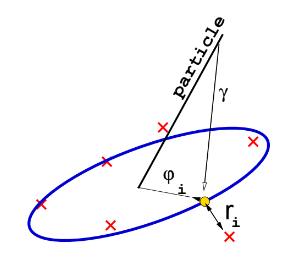
\includegraphics{Tesis-UNAM/Capitulo3/likelihoodAMS.png}
    \caption{Ilustración tomada de \cite{Ypsilantis:2003fs}}
    \label{fig:enter-label}
\end{figure}

La implementación utilizada por el experimento AMS-02 consiste en caracterizar la distribución de los residuales i.e. la distancia de los fotones detectados a la hipotesis\cite{barao2007amsrich, BARAO2003310}, esto debido a que con trigonometría se puede obtener el radio del anillo en función del ángulo cerenkov $r(\theta_c)$ y de la posición del centro del círculo $\phi$.

Por lo que el valor de $\theta_c$ será el obtenido al maximizar la siguiente función de verosimilitud.\cite{barao2007amsrich, BARAO2003310}

\begin{equation}
    L(\theta_c) = \prod_{i=1}^N P_i \left[ r_i(\theta_c, \phi) \right]
\end{equation}

La distribución de probabilidad dependerá de la geometría del detector y de las carcaterísticas del detector

\section{Redes Neuronales}
Las redes neuronales son el andamiaje matemático con el cuál la inteligencia artificial actual esta cimentada, en esta sección se esclarecerá el funcionamiento reduciéndolo a un problema meramente de optimización y se justificará su utilidad.\\

Debido a que las redes neuronales se pueden representar cómo grafos, podemos clasificarlas con base en la topología de su arquitectura, para este trabajo sólo se profundizará las topologías densas y convolucionales.

\subsection{Topología Totalmente Conectada}

\subsubsection{Perceptrón}
\begin{figure}[h!]
    \centering
    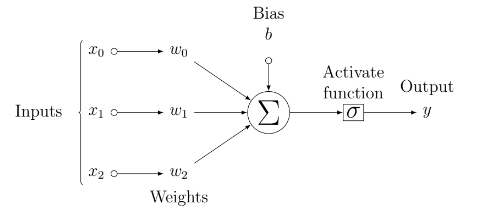
\includegraphics[scale=0.7]{Tesis-UNAM/Capitulo3/perceptron.png}
    \caption{Esquema de un perceptrón}
    \label{fig:enter-label}
\end{figure}

La neurona o perceptrón es la unidad básica de las redes neuronales. A grandes rasgos consta de una función lineal $f:\mathbb{R}^n\xrightarrow{}\mathbb{R}$ compuesta de una función no lineal, i.e. tangente hiperbólica o la función sigmoide.

\begin{equation}
    y = \sigma(w^Tx+b)
\end{equation}

Esta función de activación dota de no-linearidad al perceptrón ya que si apilamos varios perceptrones sin función de activación se obtiene una regresión lineal.\cite{Aggarwal2024DeepLearning} Y también permite constreñir el rango de la función a un intervalo en específico.

\begin{figure}[h!]
    \centering
    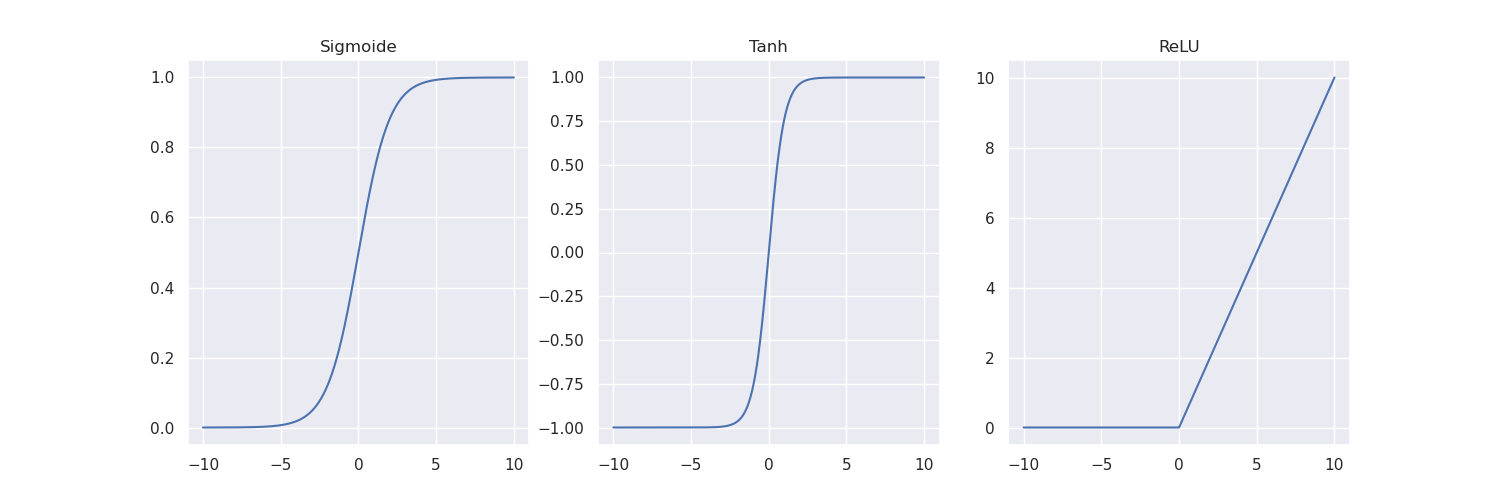
\includegraphics[scale=0.4]{Tesis-UNAM/Capitulo3/Activacion.png}
    \caption{Las funciones de activación más comunes}
    \label{fig:enter-label}
\end{figure}
\subsubsection{Redes Densas}
La razón de por que las redes neuronales son tan utiles para una amplia gama de tareas, es debido a poder apilar varias neuronas, o inclusive conectar varias capas de más de una neurona entre si.\\\\
Se puede demostrar matematicamente que cualquier funcíon se puede aproximar perfectamente con un numero infinito de perceptrones\cite{Aggarwal2024DeepLearning}. Debido a que el coste computacional de tener una infinidad de neurones es enorme, utilizar estas redes sería inmposible. A fortunadamente las redes con miles o inclusive millones de parametros dan muy buenos resultados y gracias a las modernas GPU's se puede entrenar un modelo bastante poderoso en menos de un día\\

Una de las topologías más comunes es conectar todas las neuronas de una capa con todas la neuronas de la siguiente capa.\\

Para este tipo de redes podemos calcular dada una evaluación de una neurona $x^{\left( k-1 \right)}$ de una capa previa con $n_{k-1}$ neuronas, la evaluación de un neurona i de la actual capa $x_i^{\left( k \right)}$ con $n_k$ neuronas mediante la ecuación.\cite{Aggarwal2024DeepLearning, Beyer}

\begin{equation}
    x_i^{\left( k \right)} = \sigma \left( \sum_{j=1}^{n^{\left( k-1 \right)}} w_{ji}^{\left( k \right)}x_j^{\left(k-1 \right)} + b_i^{\left( k\right)}\right) = \sigma(z_i^{(k)})
\end{equation}

\begin{figure}
    \centering
    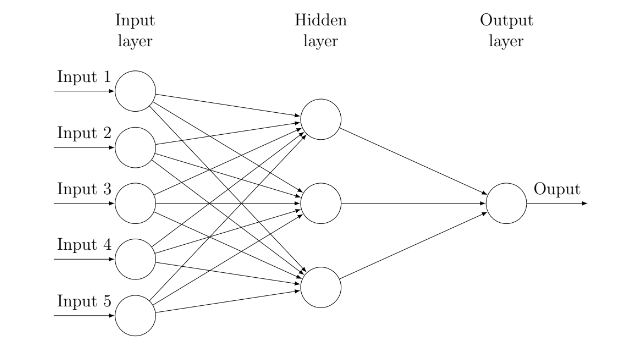
\includegraphics[scale=0.7]{Tesis-UNAM/Capitulo3/Red.png}
    \caption{Red totalmente conectada o densa}
    \label{fig:enter-label}
\end{figure}

\subsubsection{Propagación Hacia Atrás}
La razón por la cual estos modelos se denominan Inteligencia Artificial es debido a la capacidad de corregirse a si mismos y poder por ejemplo, entender un texto, o transcribir un audio sin tener que programar explicitamente todas estas funciones, esto es gracias al algoritmo de propagación hacia atrás.\\

Este algoritmo consiste en modificar los parámetros de la red neuronal con la intención de encontrar el mínimo global de una función error, esto se puede lograr usando el algoritmo de descenso del grádiente ya que el negativo del gradiente apunta en la dirección de descenso más empinado.\\

Para una función $L:\mathbb{R}^n\xrightarrow{} \mathbb{R}$ y una constante $\gamma \in \mathbb{R}^+$ llamada tasa de aprendizaje el algoritmo es el siguiente, rnd se refiere a un punto aleatorio y $\epsilon$ un infinitesimal

\begin{algorithm}
    \caption{Propagación Hacia Atrás}\label{alg:cap}
    \begin{algorithmic}
    \State $\gamma \gets \gamma$
    \State $n_{iter} \gets n_{iter}$
    \State $p_0 \gets rnd$
    \State $tol \gets \epsilon$
    \While{$i<n_{iter}$}
        \State{$p_{i+1} \gets p_{i}-\gamma\nabla L$}
        \If{$d(p_{i+1}, p_{i})>tol$}
        \State $i \gets i+1$
        \EndIf
        \EndWhile
    \end{algorithmic}
\end{algorithm}

Una vez definido el algoritmo tenemos que relacionar el gradiente con los parámetros de la red neuronal, para esto tenemos que derivar el error con respecto a los pesos y posteriormente usar la regla de la cadena \cite{Beyer}

\begin{equation}
    \frac{\partial L}{\partial w_{ij}^{(k)}} = \frac{\partial L}{\partial x_j^{(k)}}\frac{\partial x_j^{(k)}}{\partial z_j^{(k)}}
    \frac{\partial z_j^{(k)}}{\partial w_{ij}^{(k)}}
\end{equation}

Usando la ecuación 3.4 podemos obtener las siguientes relaciones
$$
    \frac{\partial z_j^{(k)}}{\partial w_{ij}^{(k)}} = x_i^{(k-1)}
$$
$$
    \frac{\partial x_j^{(k)}}{\partial z_j^{(k)}} = \sigma'(z_j^{(k)})
$$

Con este algoritmo de propagación atrás podemos hacer de manera iterativa

\begin{equation}
    w_{ij}^{(k)} \xrightarrow{} w_{ij}^{(k)} - \gamma \frac{\partial L}{w_{ij}^{(k)}}
\end{equation}

Actualmente se utilizan diferentes variaciones de este algoritmo pero en principio siguen queriendo obtener un mínimo de una función de error utilizando el descenso del gradiente.\cite{Aggarwal2024DeepLearning, Beyer}

\begin{figure}[h!]
    \centering
    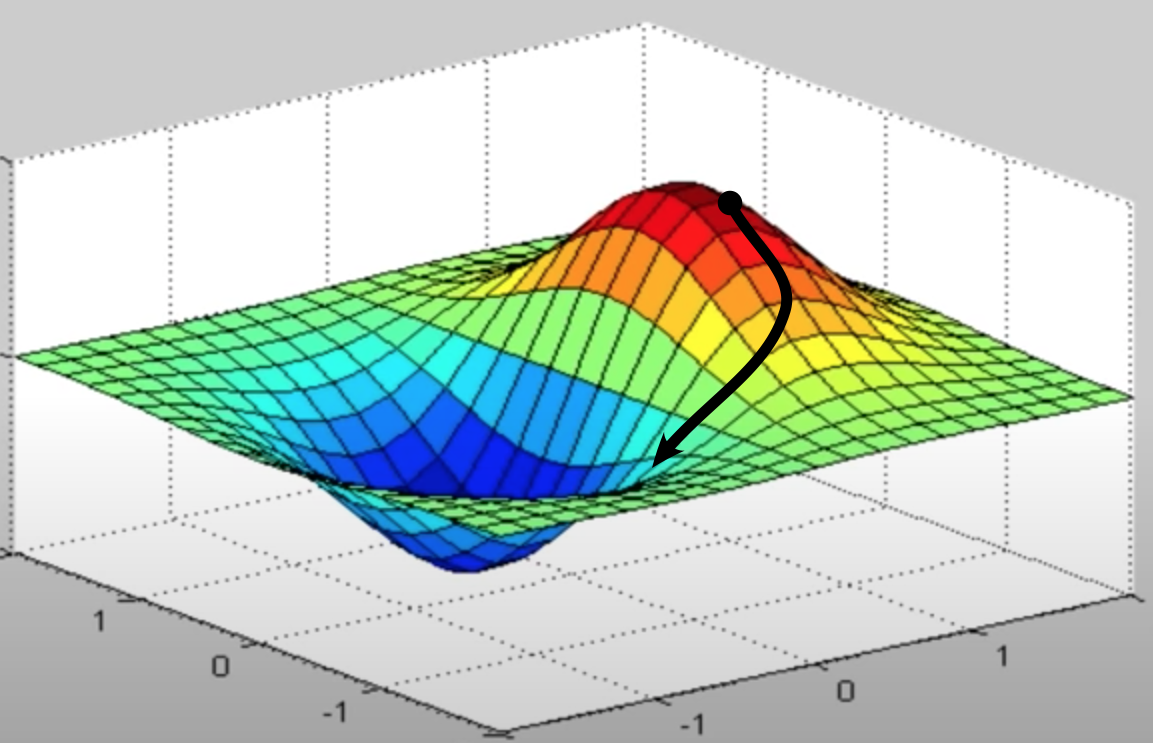
\includegraphics[scale=0.21]{Tesis-UNAM/Capitulo3/gradient.png}
    \caption{Ilustráción gráfica del algoritmo}
    \label{fig:enter-label}
\end{figure}

\subsubsection{Funciones de Error}
El proceso de entrenamiento consiste en disminuir el error de datos previamente ya conocidos proveyendo de retroalimentación al modelo, en este trabjo se utilizó la función de error más común para problemas de regresión, el error promedio al cuadrado\cite{Aggarwal2024DeepLearning}

$$ MSE = \frac{1}{N}\sum_{i=1}^{N}(y-\hat{y})^2$$

y es el valor estimado por el modelo de IA, y $\hat{y}$  es el valor real previamente conocido, esta función es diferenciable pero dominan bastante más los errores grandes.\cite{Beyer}

\subsubsection{Entrenamiento del Módelo}
El entrenamiento del modelo consiste en varias épocas, una epoca es una fase en la cuál todos los datos son utilizados en el entrenamiento, 
y una época consta de diferentes lotes, generalmente son de múltiplos de 8 debido a la arquitectura de las GPU's, y es al final de cada lote que se modifican los parámetros de la red utilizando el algoritmo de propagación hacia atrás.\\

Debido a que se busca prevenir el sobreajuste a los datos de entrenamiento, causando una falla en la predicción de data nueva, se aparta una pequeña parte de los datos para evaluar el modelo al final de cada epoca y corroborar que el error de este lote de validación no seaa mayor al error del entrenamiento (lo que indicaría un sobreajuste del modelo)

\subsection{Toplogía Convolucional}
Las imágenes computacionales se representan en pixeles, en imágenes de blanco y negro el pixel representa varias tonalides grisaceas, esto se puede ver cómo un mapeo del pixel al intervalo $\left[0, 1\right]\in \mathbb{R}$ donde cero representa el blanco y uno el negro. Cuando las imágenes son a color esto se puede hacer de una manera similar, ya que todos los colores se representan con combinaciones de rojo, azul, y verde, así que en este caso el pixel se mapea al subespacio $\left[0, 1\right] \times \left[0, 1\right] \times \left[0, 1\right] \in \mathbb{R}^3$ donde cero representa la ausencia del color en el pixel y uno la saturación total, cada intervalo cerrado necesario para representar la imagen se denomina canal.\\

Por lo tanto las imágenes son matrices, no vectores, ya que un vector no representaria fielmente la localización del pixel con respecto a la imagen, esto hace que querer usar una red densa no sea lo más eficiente y además no sería invariante al desplazamiento\cite{LeCun1998GradientbasedLA}, e.g. si tenemos una esquina, las neuronas que hayan detectado esta esquina sólo podrían identificarla en la misma posición original, no podría detectar la misma esquina en otro lugar de la imagen.\\

\begin{figure}[h!]
    \centering
    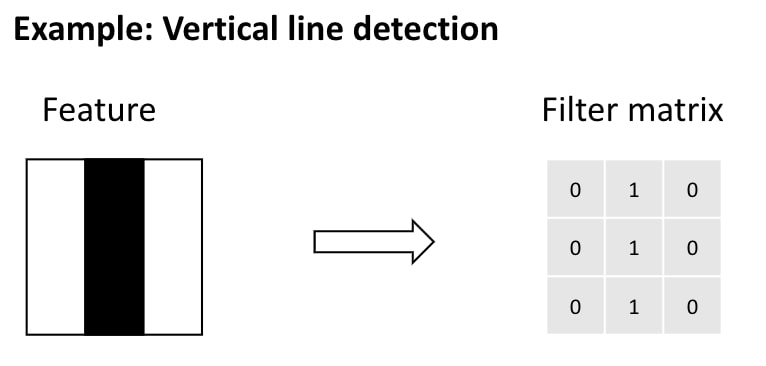
\includegraphics[scale=0.6]{Tesis-UNAM/Capitulo3/filtrosjpeg.jpeg}
    \caption{Filtro capaz de detectar líneas verticales}
    \label{fig:enter-label}
\end{figure}

LeCun en 1998 estudió el árticulo de Hubel y Weisel en donde se descubrió las neuronas del sistema visual de los gatos\cite{LeCun1998GradientbasedLA}, y desarrolló una nueva arquitecura de redes neuronales la cuál denominó convolucional.\\

Esta arquitectura presenta invarianza al desplazamiento al convolucionar filtros sobre toda la imagen. Los filtros son matrices de una dimensión mucho menor a la imagen y que sirven para detectar esquinas, líneas rectas, diagonales, etc... Estos filtros serían los parámetros de la red neuronal a entrenar.\\

\begin{figure}[h!]
    \centering
    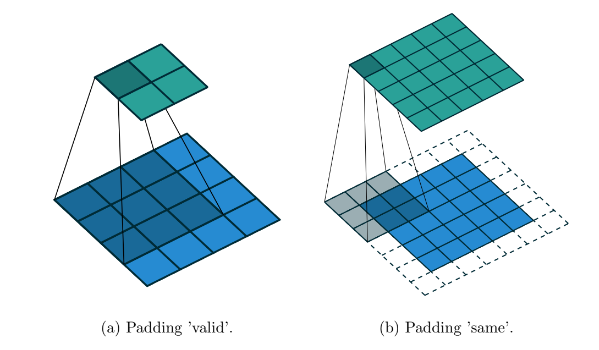
\includegraphics[scale=0.75]{Tesis-UNAM/Capitulo3/padding.png}
    \caption{Los cuadros azules representan la data original y los transparentes los valores añadidos en el padding. \cite{Beyer}}
    \label{fig:enter-label}
\end{figure}

La razón de llamarse redes convolucionales es que estos filtros se convolucionan con la imagen, detectando patrones en la imagen entera y respetando la invarianza al desplazamiento de los mismos.También hay que aclarar que de esta manera se obtiene un rendimiento mucho mayor con un número bastante menor de parametros con respecto a una topología totalmente conectada.\cite{LeCun1998GradientbasedLA}\\

Cómo los anillos cerenkov se pueden representar a blanco y negro, se utilizará sólo un canal. Al realizar la convolución de los filtros con la imagen se obtiene mediante la siguiente ecuación, con k un filtro.\cite{Beyer}

\begin{equation}
    y_{a, b} = \sum_{i=-u}^u\sum_{j=-u}^uk_{i,j}x_{a+i,b+j}+B
\end{equation}

Con a, b los índices del pixel de la imagen, y un tamaño de filtro $f\timesf=(2u+1)\times(2u+1)$ impar, además cada filtro contiene un valor de sezgo B, finalmente a la convolución resultante se le aplíca una función de activación.

\subsubsection{Padding y Striding}
Debido a que la operación convolución puede reducir la dimensionalidad de la imagen, al conectar varias capas convolucional podemos inclusive reducir la imagen a una matriz de un sólo elemento. Una forma de solucionar este problema es incluyendo padding en cada capa convolucional.\\

\begin{figure}[h!]
    \centering
    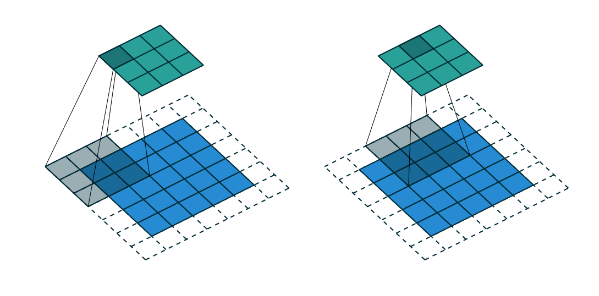
\includegraphics[scale=0.75]{Tesis-UNAM/Capitulo3/stridding.png}
    \caption{Dos convoluciones seguidos con un stridding de 2 en el eje x y padding "same". \cite{Beyer} }
    \label{fig:enter-label}
\end{figure}

Este padding le añade pixeles a la frontera de los datos con ceros u otros valores predichos. Los frameworks de IA más usados contienen opciones predefinidas, cómo "same" que mantiene el tamaño antes de la convolución; o "valid" que añade sólo los valores necesarios para que pueda ser correcta la convolución.\\

También existe el "stridding" lo que define el tamaño del desplazamiento en píxeles durante cada operación de convolución, puede ser uno, o dos píxeles por ejemplo, y también variar el tamaño si el desplazamiento es en el eje x o y, e.g. dos horizontales y uno vertical. Esto puede reducir la dimensión de la data pero hay momentos donde llega a ser beneficioso, por ejemplo si se busca optimizar la velocidad de entrenamiento del modelo, reduciendo el número de parámetros a entrenar conforme se avanza en la red neuronal.\\
      % ~20 páginas - Explicar el problema en específico que se va a resolver, la metodología y experimentos/métodos utilizados
\chapter{Análisis de Resultados}

%Section describiendo la simulación
%Geant4, ROOT y describiendo la geometría, las condiciones iniciales, materiales, etc.


\section{Configuración Perpendicular}
\subsection{Likelihood}
\begin{figure}
    \centering
    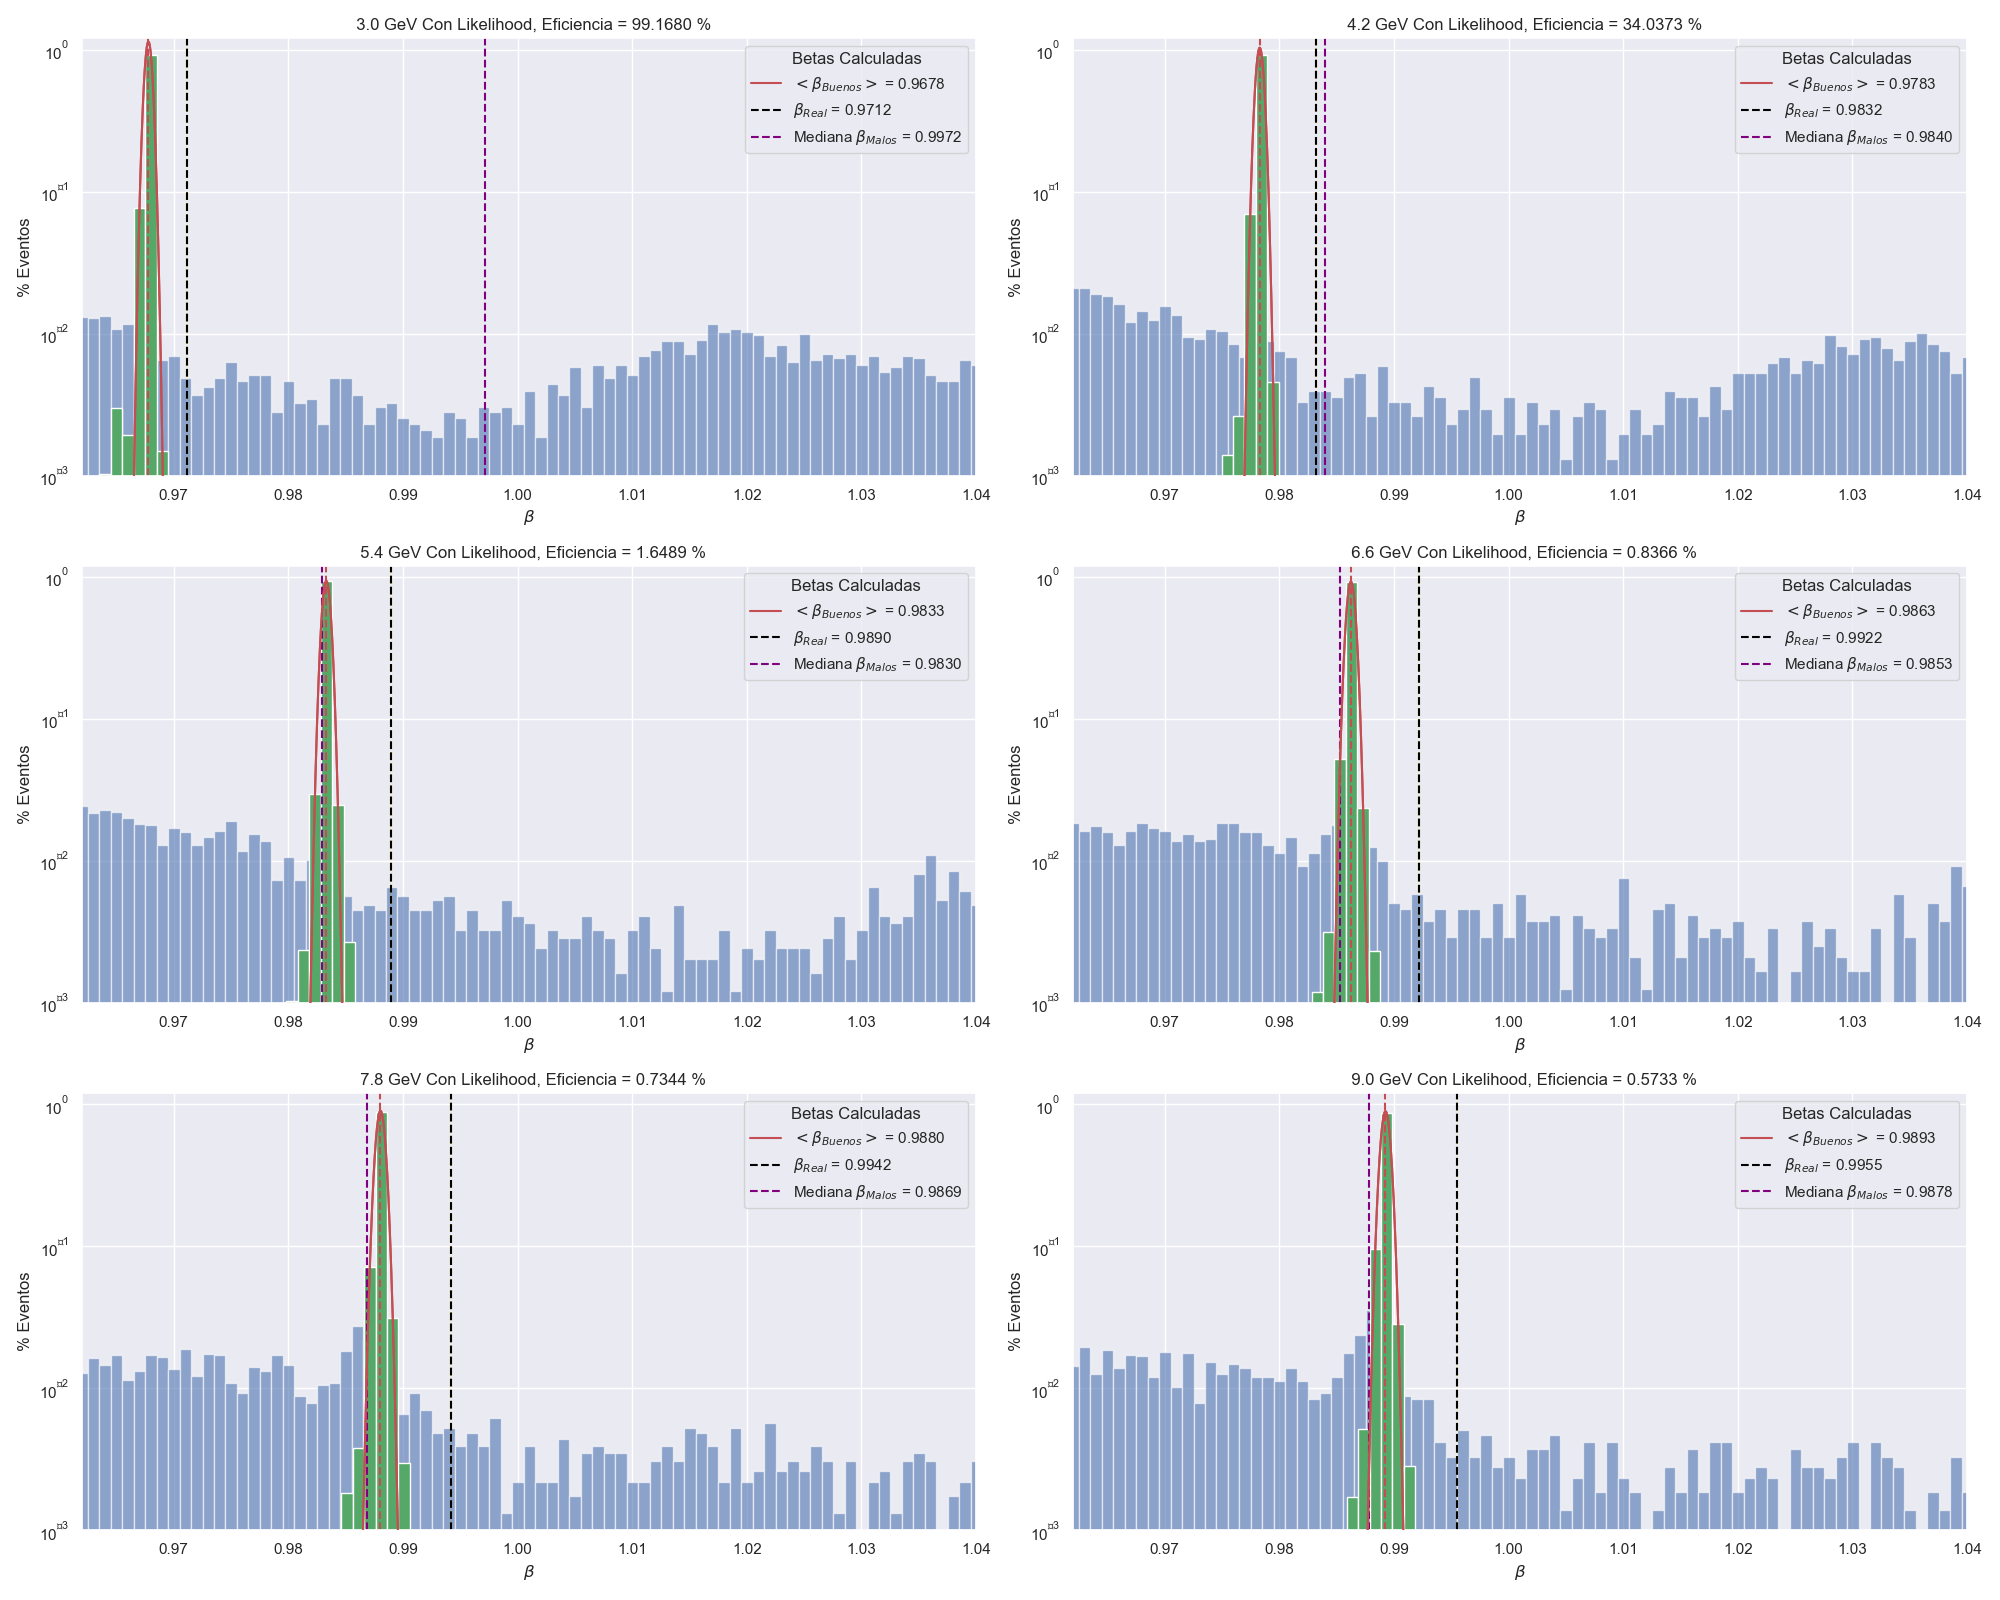
\includegraphics[width=18cm, height=21cm, left]{Tesis-UNAM/Capitulo4/pLike9.png}
    \caption{La eficiencia se refiere al porcentaje de eventos en el rango de 0.5\% con respecto a la beta real}
    \label{fig:enter-label}
\end{figure}

\boxed{$$f(x) = \begin{cases} 
          \frac{1}{\sigam 2\pi}exp\left( -\frac{1}{2}\frac{(x-\mu)^2}{\sigma^2} \right) & x \leq x_0 \\
           a_1\left(\frac{x}{x_0}\right)^{k_1} & x_0 \leq x\\
       \end{cases}
$$}

\begin{figure}
    \centering
    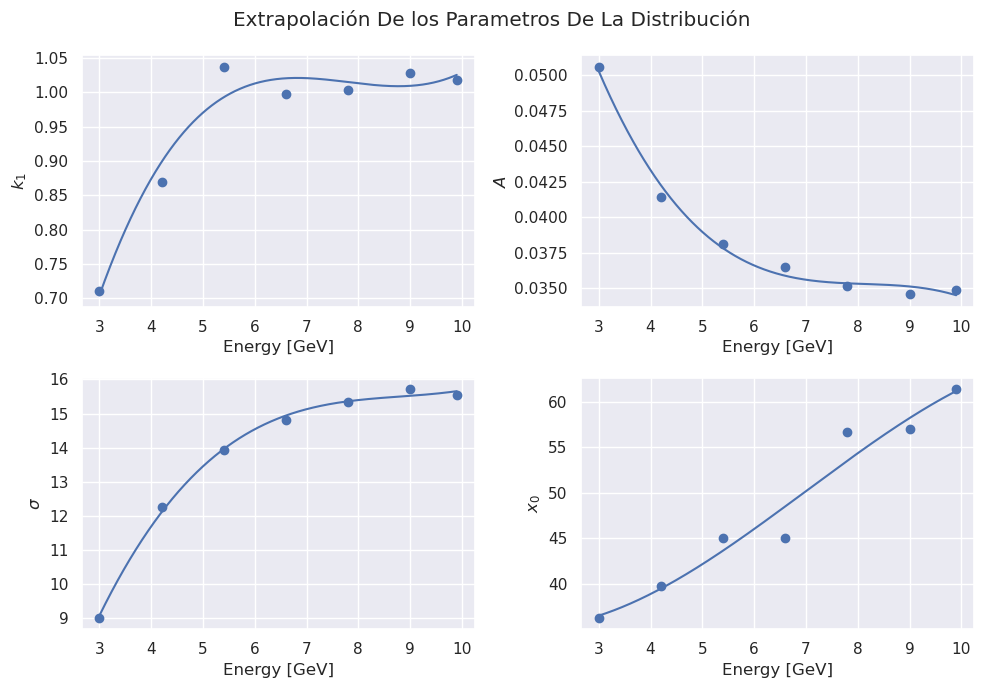
\includegraphics[width=12cm]{Tesis-UNAM/Capitulo4/parametros.png}
    \caption{Parámetros De La Distribución a Ajustar}
    \label{fig:enter-label}
\end{figure}

\begin{figure}
    \centering
    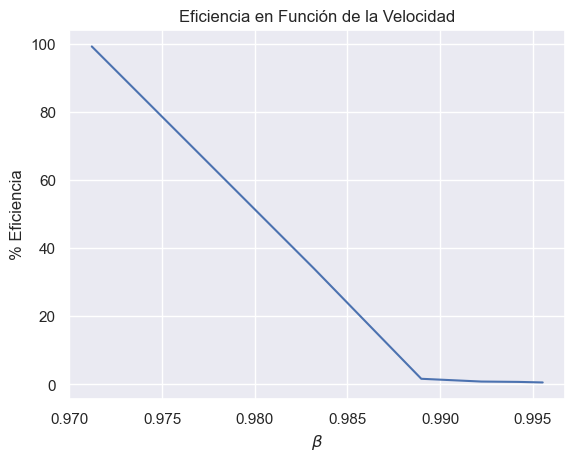
\includegraphics[scale=0.6]{Tesis-UNAM/Capitulo4/EficienciaLike.png}
    \caption{9cm Aerogel}
    \label{fig:enter-label}
\end{figure}

\begin{figure}
    \centering
    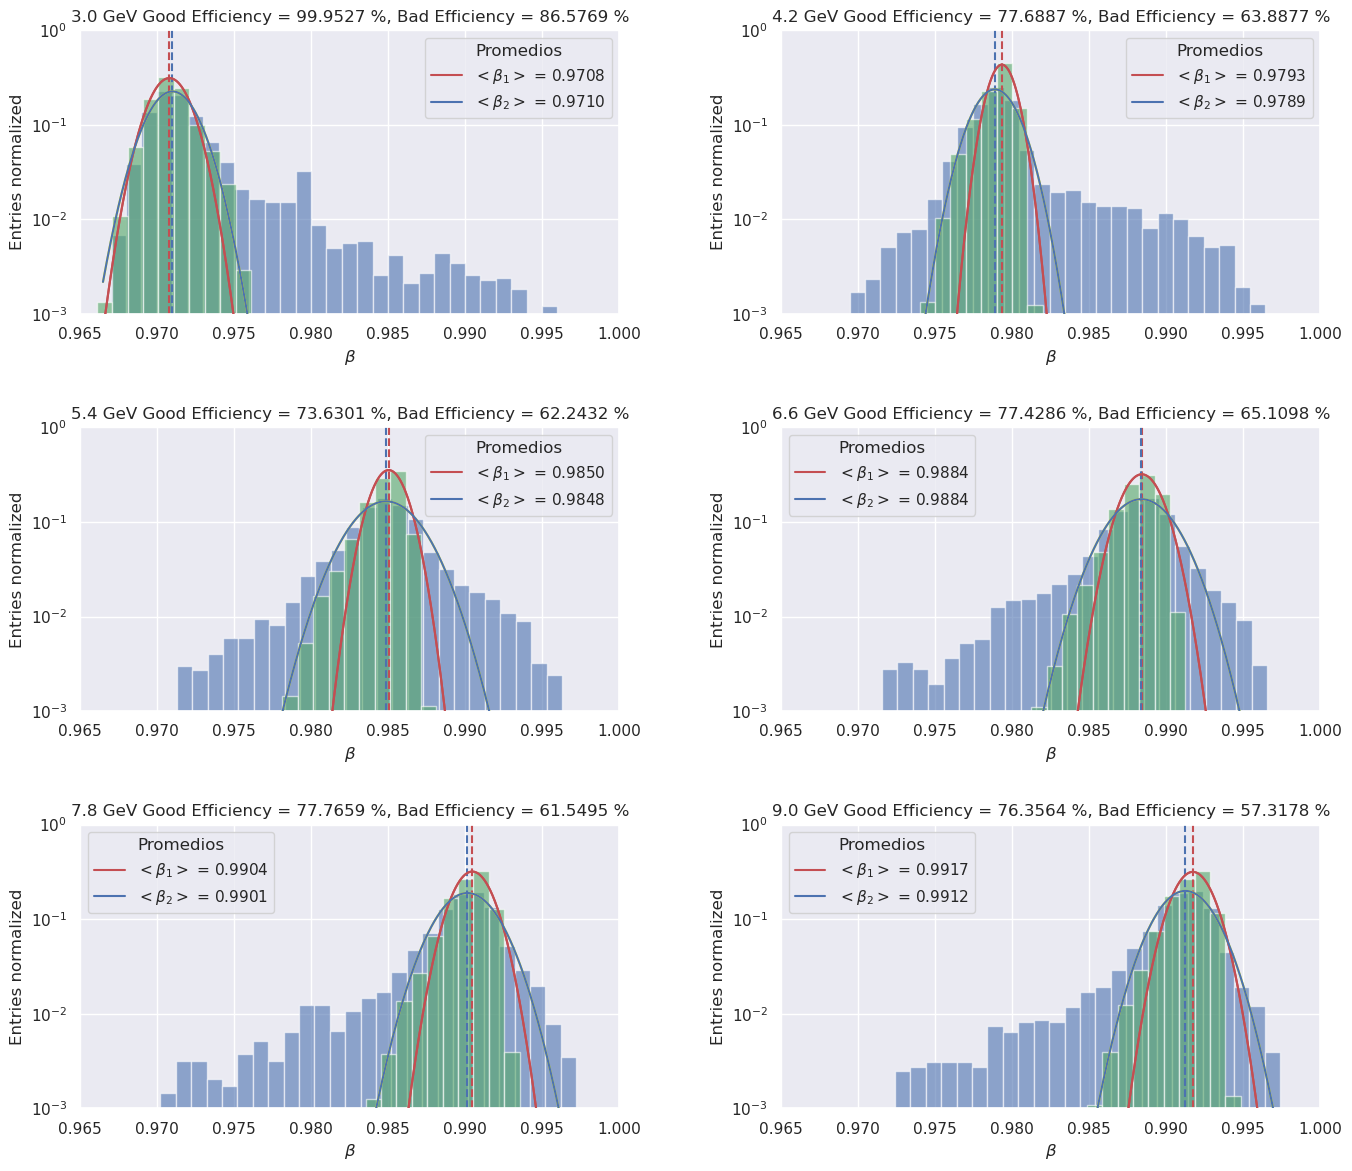
\includegraphics[width=15cm, height=21cm]{Tesis-UNAM/Capitulo4/9pAI.png}
    \caption{9cm Aerogel}
    \label{fig:enter-label}
\end{figure}

\begin{figure}
    \centering
    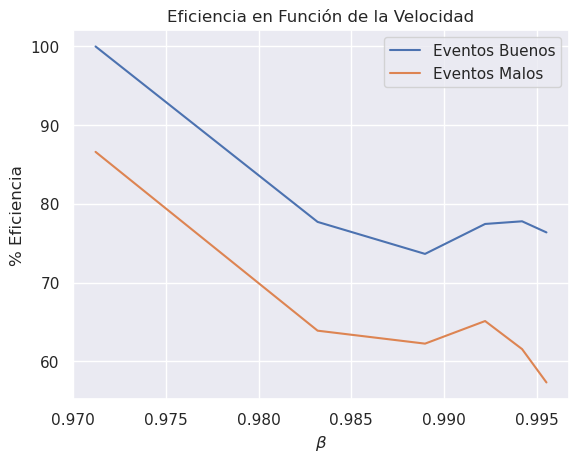
\includegraphics[scale=0.6]{Tesis-UNAM/Capitulo4/EficienciaAI.png}
    \caption{9cm Aerogel}
    \label{fig:enter-label}
\end{figure}
\subsection{Redes Neuronales}
\subsection{Comparación}
\section{Configuración Multidireccional}
\subsection{Likelihood}
\subsection{Redes Neuronales}
\subsection{Comparación}   % ~20 páginas - Presentar los resultados tal cual son, y analizarlos.
\chapter{Conclusiones}
\blindtext            % ~5 páginas - Resumir lo que se hizo y lo que no y comentar trabajos futuros sobre el tema

%%%%%%%%%%%%%%%%%%%%%%%%%%%%%%%%%%%%%%%%%%%%%%%%%%%%%
%                   APÉNDICES                       %
%%%%%%%%%%%%%%%%%%%%%%%%%%%%%%%%%%%%%%%%%%%%%%%%%%%%%
\appendix
% this file is called up by thesis.tex
% content in this file will be fed into the main document
\chapter{Código/Manuales/Publicaciones}
% top level followed by section, subsection

\section{Apéndice}

Apéndice
               % Colocar los circuitos, manuales, código fuente, pruebas de teoremas, etc.

%%%%%%%%%%%%%%%%%%%%%%%%%%%%%%%%%%%%%%%%%%%%%%%%%%%%%
%                   REFERENCIAS                     %
%%%%%%%%%%%%%%%%%%%%%%%%%%%%%%%%%%%%%%%%%%%%%%%%%%%%%
% existen varios estilos de bilbiografía, pueden cambiarlos a placer
\bibliographystyle{apalike} % otros estilos pueden ser abbrv, acm, alpha, apalike, ieeetr, plain, siam, unsrt

%El formato trae otros estilos, o pueden agregar uno que les guste:
%\bibliographystyle{Latex/Classes/PhDbiblio-case} % title forced lower case
%\bibliographystyle{Latex/Classes/PhDbiblio-bold} % title as in bibtex but bold
%\bibliographystyle{Latex/Classes/PhDbiblio-url} % bold + www link if provided
%\bibliographystyle{Latex/Classes/jmb} % calls style file jmb.bst

\bibliography{Bibliografia/referencias}             % Archivo .bib


\end{document}
